\documentclass[a4paper, 12pt]{article}
\usepackage[a4paper,top=1.5cm, bottom=1.5cm, left=1cm, right=1cm]{geometry}
\usepackage[utf8]{inputenc}
\usepackage{mathtext}
\usepackage{amsmath}
\usepackage{amsfonts}
\usepackage[english, russian]{babel}
\usepackage{indentfirst}
\usepackage{longtable}
\usepackage{graphicx}
\graphicspath{{pictures/}}
\DeclareGraphicsExtensions{.pdf,.png,.jpg}
\usepackage{natbib}
\usepackage{mathrsfs}
\usepackage[europeanresistors, americaninductors]{circuitikz}

\title{Лабораторная работа 1.1.1 Определение систематических и случайных погрешностей при измерении удельного сопротивления нихромовой проволоки}
\author{Михаил Колтаков}
\date{21 сентября 2020 г.}

\begin{document}
	\maketitle
	\section*{Цель работы}
		Измерить удельное сопротивление проволоки и вычислить систематические и случайные погрешности при использовании таких измерительных приборов, как линейка, штангенциркуль, микрометр, амперметр, вольтметр и мост постоянного тока
	\section*{Оборудование}
		Линейка, штангенциркуль, микрометр, отрезок проволоки из нихрома, амперметр, вольтметр, источник ЭДС, мост постоянного тока, реостат
	\section*{Теория к работе}
		На протяжении всей работы
		
		$\rho - удельное\: сопротивление\: нихрома$
		
		$d - диаметр\: проволоки$
		
		$l - длина\: измеряемого\: участка\: проволоки$
		
		$R_{пр} - сопротивление\: проволоки$
		
		$R_A - сопротивление\: амперметра$
		
		$R_V -  сопротивление\: вольтметра$
		
		$R - сопротивление\: реостата$
		
		$\mathscr{E} - ЭДС\: источника$
		
		$V - показание\: вольтметра$
		
		$I - показание\: амперметра$
		\par
		Удельное сопротивление нихрома можно вычислить по формуле
		$$\rho = \frac{R_{пр}\pi d^2}{4l}$$\\
		\\
		\\
		\\
		\\
		\\
		
		В работе мы использовали схему установки a), так как она даёт нам меньшую погрешность при измерении сопротивления проволоки($1,25\cdot10^{-3}$ против 0,24)\\
		
		\begin{circuitikz}
			\draw (4.25, 0) to [pR, -., mirror, l=$R$, name=P] (3.1, 0)
			to [battery1, -., l=$\mathscr{E}$] (1, 0)
			to [rmeter, t=A] (1, -1.25)
			to [R, l=$R_A$] (1, -2.5)
			to (1, -4)
			to [rmeter, t=V] (2.5, -4)
			to [R, l=$R_V$] (4, -4)
			to (4.5, -4)
			to [nos] (4.5, 0)
			to (4.25, 0);
			\draw (3, 0) to [short] (2.8, 0) to [short] (2.8, 0.558) to (P.wiper);
			\draw (1, -3) to [R, l=$R_{пр}$] (4.5, -3) to (4.5, -3);
			\draw (1, -3) node[circ]{}
			(4.5, -3) node[circ]{};
		\end{circuitikz}
		\par
		В этом случае сопротивление проволоки с поправкой на сопротивление приборов можно рассчитывать по формуле
		$$R_{пр} = \frac{R_V}{R_V-R_{пр}^и}$$
		$R_{пр}^и - измеренное\: сопротивление\: проволоки$
		\\
		
		Необходимо также произвести расчёт систематической и случайной погрешности измерений толщины проволоки и показаний амперметра с вольтметром.
		Опыт будем проводить для трёх длин проволоки(20 см, 30 см и 50 см)
		
		Строим ВАХи для всех отрезков проволоки, после этого оцениваем погрешности измерения среднего сопротивления проволоки с помощью МНК.
	\section*{Ход работы}
		1. Точность измерения с помощью штангенциркуля - 0,1 мм. Точность измерения с помощью микрометра - 0,01 мм.
		\par
		2. Измеряем толщину проволоки штангенциркулем($d_1$) и микрометром($d_2$) на 10 различных участках.
		\begin{longtable}[H]{|c|c|c|c|c|c|c|c|c|c|c|}
			\hline
			& 1 & 2 & 3 & 4 & 5 & 6 & 7 & 8 & 9 & 10 \\
			\hline
			$d_1, мм$ & 0,4 & 0,4 & 0,4 & 0,4 & 0,4 & 0,4 & 0,4 & 0,4 & 0,4 & 0,4 \\
			\hline
			$d_2, мм$ & 0,36 & 0,36 & 0,35 & 0,35 & 0,35 & 0,34 & 0,35 & 0,35 & 0,35 & 0,35 \\
			\hline
			& \multicolumn{10}{c|}{$\overline{d_1} = 0,4\: мм \;\;\; \overline{d_2} = 0,35\: мм$} \\
			\hline
		\end{longtable}
		При измерении диаметра проволоки штангенциркулем случайная погрешность отсутствует, значит, можно учитывать только систематическую, которая является точностью штангенциркуля
		$$d_1 = (0,4 \pm 0,1)\: мм$$
		
		Измерения с помощью микрометра содержат как систематическую, так и случайную погрешности:
		$$\sigma_{сист}=0,01\: мм,\;\;\;\;\;\; \sigma_{сл}=\frac{1}{N} \sqrt{\sum_{i=1}^{n}(d_i - \overline{d})^2}=\frac{1}{10} \sqrt{2,9\cdot 10^{-4}}\approx 1,7\cdot 10^{-3} мм$$
		$$\sigma_d = \sqrt{\sigma_{сист}^2+\sigma_{сл}^2}\approx 0,01 мм$$
		Поскольку $\sigma_{сл}^2 \ll \sigma_{сист}^2$, то можно считать проволоку однородной по диаметру, а погрешность диаметра $\sigma_d$ определяется только $\sigma_{сист}$ микрометра.
		$$d_2=\overline{d_2} \pm \sigma_d = (0,35 \pm 0,01)\: мм$$
		\par
		3. Определим площадь поперечного мечения проволоки:
		$$S = \frac{\pi d_2^2}{4}=\frac{3,14\cdot(0,35)^2}{4}\approx 9,62\cdot 10^{-2}\:  мм^2$$
		Величину погрешности измерения площади $\sigma_S$ найдём по формуле
		$$\sigma_S=2\frac{\sigma_d}{d}S=2\frac{0,01}{0,35}\cdot 9,62\cdot 10^{-2}=5\cdot 10^{-4}\: мм$$
		Итак, $S=(9,62 \pm 0,04)\cdot 10^{-2}\: мм^{2}$, т. е. площадь поперечного сечения проволоки определена с точностью $0,4\%$
		\par
		4. Сведём характеристики приборов в таблицу
		\begin{longtable}[H]{|c|c|c|c|}
			\hline
			& Вольтметр & Миллиамперметр & Мост \\
			\hline
			Система & Магнитоэлектрическая & Электромагнитная & --- \\
			Класс точности & 0,2 & 0,2 & 0,1 \\
			Предел измерений $x_П$ & 0,6 В & 0,5 А & --- \\
			Число делений шкалы $n$ & 150 & --- & --- \\
			Цена делений $x_П/n$ & 4 мВ/дел & --- & --- \\
			Чувствительность $x_П/n$ & 250 дел/В & --- & --- \\
			Абсолютная погрешность $\Delta x_М$ & 2 мВ & 0,62 мА & --- \\
			Внутреннее сопротивление прибора & 4000 Ом & 1,6 Ом & --- \\
			\hline
		\end{longtable}
		\par
		6. Собираем схему 1a).
		\par
		7. Опыт проводим для $l_1=(20,0 \pm 0,1)\: см; l_2=(30,0 \pm 0,1)\: см; l_3=(50,0 \pm 0,1)\: см$
		
		Результаты измерений заносим в таблицу
		\begin{longtable}[H]{|c|c|c||c|c|c||c|c|c|}
			\hline
			\multicolumn{3}{|c||}{$l = 20\: см$} & \multicolumn{3}{c||}{$l = 30\: см$} & \multicolumn{3}{c|}{$l = 50\: см$}  \\
			\hline
			V, дел  4 мВ/дел & V, мВ & I, мА & V, дел  4 мВ/дел & V, мВ & I, мА & V, дел  4 мВ/дел & V, мВ & I, мА \\
			\hline
			150 & 600 & 292 & 150 & 600 & 192 & 151 & 604 & 115 \\
			\hline
			131 & 524 & 255 & 142 & 568 & 182 & 142 & 568 & 108 \\
			\hline
			120 & 480 & 233 & 118 & 472 & 151 & 130 & 520 & 99 \\
			\hline
			115 & 460 & 224 & 106 & 424 & 136 & 124 & 496 & 95 \\
			\hline
			110 & 440 & 215 & 93 & 372 & 118 & 109 & 436 & 83 \\
			\hline
			100 & 400 & 194 & 80 & 320 & 102 & 101 & 404 & 77 \\
			\hline
			90 & 360 & 175 & 69 & 276 & 89 & 99 & 396 & 75 \\
			\hline
			85 & 340 & 165 & 62 & 248 & 80 & 89 & 356 & 68 \\
			\hline
			80 & 320 & 155 & 56 & 224 & 72 & 77 & 308 & 59 \\
			\hline
			70 & 280 & 136 & 50 & 200 & 64 & 70 & 280 & 53 \\
			\hline
			60 & 240 & 117 & 44 & 176 & 57 & 61 & 244 & 47 \\
			\hline
			55 & 220 & 108 & 39 & 156 & 50 & 41 & 164 & 31 \\
			\hline
			50 & 200 & 99 & 26 & 104 & 34 & 38 & 152 & 29 \\
			\hline
			40 & 160 & 77 & 22 & 88 & 28 & 32 & 128 & 24 \\
			\hline
		\end{longtable}
		8. Построим графики по таблице(В конце документа).
		\par
		9. Для каждой длины $l$ проводим расчёт методом наименьших квадратов и вычислим погрешность по формулам
		$$ R_{ср} = \frac{\langle VI \rangle}{\langle I^2 \rangle}$$
		$$\sigma_{R_{ср}}^{случ} = \frac{1}{\sqrt{14}} \sqrt{\frac{\langle V^2 \rangle}{\langle I^2 \rangle} - R_{ср}^{2}} $$
		Возможную систематическую погрешность $R_{ср}$ оцениваем по формуле
		$$\frac{\sigma_{R_{ср}}^{сист}}{R_{ср}}=\sqrt{(\frac{\sigma_V}{V})^2+(\frac{\sigma_I}{I})^2}$$
		$I$ и $V$ - максимальные значения тока и напряжения в ходе измерений(), $\sigma_V$ и $\sigma_I$ - ошибки измерения вольтметром и амперметром: $\sigma_V = 1 мВ, \sigma_I = 0,31 мА$. Делаем поправку для нашей схемы.
		\begin{longtable}[H]{|c||c||c|}
			\hline
			$l = 20\: см$ & $l = 30\: см$ & $l = 50\: см$ \\
			\hline
			$R_0 = 2,155\: Ом$ & $R_0 = 3,222\: Ом$ & $R_0 = 5,346\: Ом$ \\
			$R_{ср} = 2,055\: Ом$ & $R_{ср} = 3,123\: Ом$ & $R_{ср} = 5,249\: Ом$ \\
			$R_{пр} = 2,056\: Ом$ & $R_{пр} = 3,125\: Ом$ & $R_{пр} = 5,256\: Ом$ \\
			$\sigma_R^{случ} = 0,002\: Ом$ & $\sigma_R^{случ} = 0,004\: Ом$ & $\sigma_R^{случ} = 0,006\: Ом$ \\
			$\sigma_R^{сист} = 0,004\: Ом$ & $\sigma_R^{сист} = 0,007\: Ом$ & $\sigma_R^{сист} = 0,017\: Ом$ \\
			$\sigma_R = 0,005\: Ом$ & $\sigma_R = 0,008\: Ом$ & $\sigma_R = 0,018\: Ом$ \\
			\hline
		\end{longtable}
		Более сокращённый вариант таблицы
		\begin{longtable}[H]{|c|c|c|c|}
			\hline
			l, см & 20 & 30 & 50 \\
			\hline
			$R_{пр},\: Ом$ & 2,056 & 3,125 & 5,256 \\
			\hline
			$\sigma_{R},\: Ом$ & 0,005 & 0,008 & 0,018 \\
			\hline
		\end{longtable}
		10. Сравниваем полученные результаты $R_{пр}$ с $R_0$, полученными на мосте. Результаты попадают в предел погрешностей.
		11. Определяем удельное сопротивление проволоки по формуле и погрешность. $\sigma_{\rho}$
		$$\sigma_{\rho}=\rho \sqrt{(\frac{\sigma_R}{R})^2 + (2 \frac{\sigma_d}{d})^2 + (\frac{\sigma_l}{l})^2}$$
		Занесём полученные результаты в таблицу
		\begin{longtable}[H]{|c|c|c|}
			\hline
			$l,\: см$ & $\rho, 10^{-5}\: Ом \cdot см$ & $\sigma_{\rho}, 10^{-6}\: Ом \cdot см$ \\
			\hline
			20 & 9.9 & 6 \\
			30 & 10.0 & 6 \\
			50 & 10.1 & 6 \\
			\hline
		\end{longtable}
		Окончательно: $\rho = (10,0 \pm 0,6) \cdot 10^{-5}\: Ом \cdot см$
	\section*{Вывод}
		Основной вклад в ошибку сносит погрешность при измерении диаметра проволоки, составляющая примерно $2,9\%$, однако, так как результат измерений удваивается, погрешность тоже умножается на 2, а значит, составляет примерно $5,7\%$. Поэтому при измерении сопротивления проволоки достаточна точность $3-4\%$.
		
		Полученное значение удельного сопротивления входит в допустимые значения для нихрома.
		\begin{figure}[h!]
			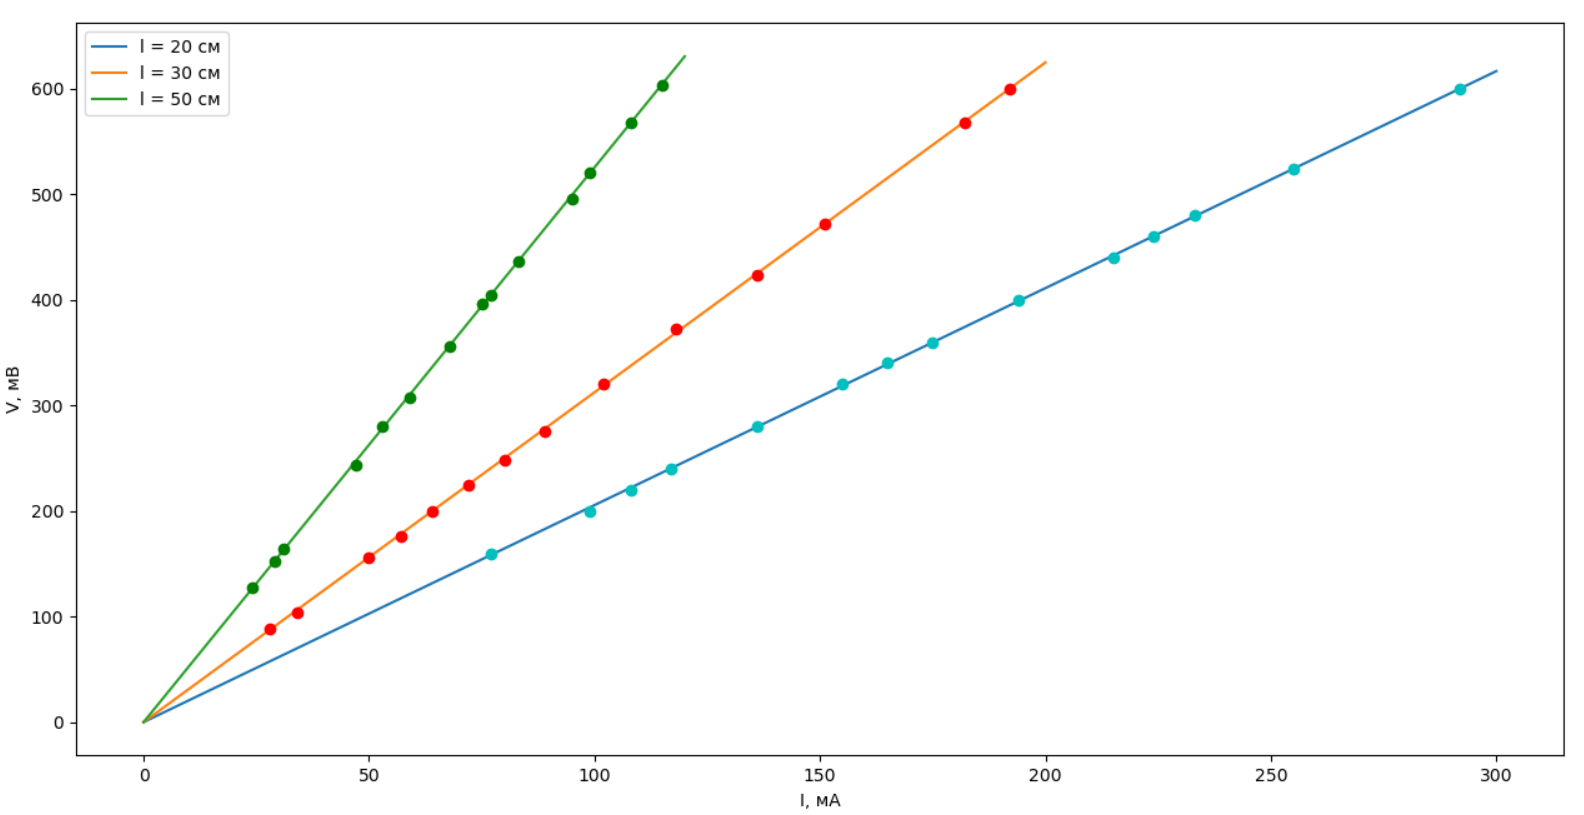
\includegraphics[width=\linewidth]{pict1}
		\end{figure}
\end{document}
